\documentclass[1p]{elsarticle_modified}
%\bibliographystyle{elsarticle-num}

%\usepackage[colorlinks]{hyperref}
%\usepackage{abbrmath_seonhwa} %\Abb, \Ascr, \Acal ,\Abf, \Afrak
\usepackage{amsfonts}
\usepackage{amssymb}
\usepackage{amsmath}
\usepackage{amsthm}
\usepackage{scalefnt}
\usepackage{amsbsy}
\usepackage{kotex}
\usepackage{caption}
\usepackage{subfig}
\usepackage{color}
\usepackage{graphicx}
\usepackage{xcolor} %% white, black, red, green, blue, cyan, magenta, yellow
\usepackage{float}
\usepackage{setspace}
\usepackage{hyperref}

\usepackage{tikz}
\usetikzlibrary{arrows}

\usepackage{multirow}
\usepackage{array} % fixed length table
\usepackage{hhline}

%%%%%%%%%%%%%%%%%%%%%
\makeatletter
\renewcommand*\env@matrix[1][\arraystretch]{%
	\edef\arraystretch{#1}%
	\hskip -\arraycolsep
	\let\@ifnextchar\new@ifnextchar
	\array{*\c@MaxMatrixCols c}}
\makeatother %https://tex.stackexchange.com/questions/14071/how-can-i-increase-the-line-spacing-in-a-matrix
%%%%%%%%%%%%%%%

\usepackage[normalem]{ulem}

\newcommand{\msout}[1]{\ifmmode\text{\sout{\ensuremath{#1}}}\else\sout{#1}\fi}
%SOURCE: \msout is \stkout macro in https://tex.stackexchange.com/questions/20609/strikeout-in-math-mode

\newcommand{\cancel}[1]{
	\ifmmode
	{\color{red}\msout{#1}}
	\else
	{\color{red}\sout{#1}}
	\fi
}

\newcommand{\add}[1]{
	{\color{blue}\uwave{#1}}
}

\newcommand{\replace}[2]{
	\ifmmode
	{\color{red}\msout{#1}}{\color{blue}\uwave{#2}}
	\else
	{\color{red}\sout{#1}}{\color{blue}\uwave{#2}}
	\fi
}

\newcommand{\Sol}{\mathcal{S}} %segment
\newcommand{\D}{D} %diagram
\newcommand{\A}{\mathcal{A}} %arc


%%%%%%%%%%%%%%%%%%%%%%%%%%%%%5 test

\def\sl{\operatorname{\textup{SL}}(2,\Cbb)}
\def\psl{\operatorname{\textup{PSL}}(2,\Cbb)}
\def\quan{\mkern 1mu \triangleright \mkern 1mu}

\theoremstyle{definition}
\newtheorem{thm}{Theorem}[section]
\newtheorem{prop}[thm]{Proposition}
\newtheorem{lem}[thm]{Lemma}
\newtheorem{ques}[thm]{Question}
\newtheorem{cor}[thm]{Corollary}
\newtheorem{defn}[thm]{Definition}
\newtheorem{exam}[thm]{Example}
\newtheorem{rmk}[thm]{Remark}
\newtheorem{alg}[thm]{Algorithm}

\newcommand{\I}{\sqrt{-1}}
\begin{document}

%\begin{frontmatter}
%
%\title{Boundary parabolic representations of knots up to 8 crossings}
%
%%% Group authors per affiliation:
%\author{Yunhi Cho} 
%\address{Department of Mathematics, University of Seoul, Seoul, Korea}
%\ead{yhcho@uos.ac.kr}
%
%
%\author{Seonhwa Kim} %\fnref{s_kim}}
%\address{Center for Geometry and Physics, Institute for Basic Science, Pohang, 37673, Korea}
%\ead{ryeona17@ibs.re.kr}
%
%\author{Hyuk Kim}
%\address{Department of Mathematical Sciences, Seoul National University, Seoul 08826, Korea}
%\ead{hyukkim@snu.ac.kr}
%
%\author{Seokbeom Yoon}
%\address{Department of Mathematical Sciences, Seoul National University, Seoul, 08826,  Korea}
%\ead{sbyoon15@snu.ac.kr}
%
%\begin{abstract}
%We find all boundary parabolic representation of knots up to 8 crossings.
%
%\end{abstract}
%\begin{keyword}
%    \MSC[2010] 57M25 
%\end{keyword}
%
%\end{frontmatter}

%\linenumbers
%\tableofcontents
%
\newcommand\colored[1]{\textcolor{white}{\rule[-0.35ex]{0.8em}{1.4ex}}\kern-0.8em\color{red} #1}%
%\newcommand\colored[1]{\textcolor{white}{ #1}\kern-2.17ex	\textcolor{white}{ #1}\kern-1.81ex	\textcolor{white}{ #1}\kern-2.15ex\color{red}#1	}

{\Large $\underline{12a_{0876}~(K12a_{0876})}$}

\setlength{\tabcolsep}{10pt}
\renewcommand{\arraystretch}{1.6}
\vspace{1cm}\begin{tabular}{m{100pt}>{\centering\arraybackslash}m{274pt}}
\multirow{5}{120pt}{
	\centering
	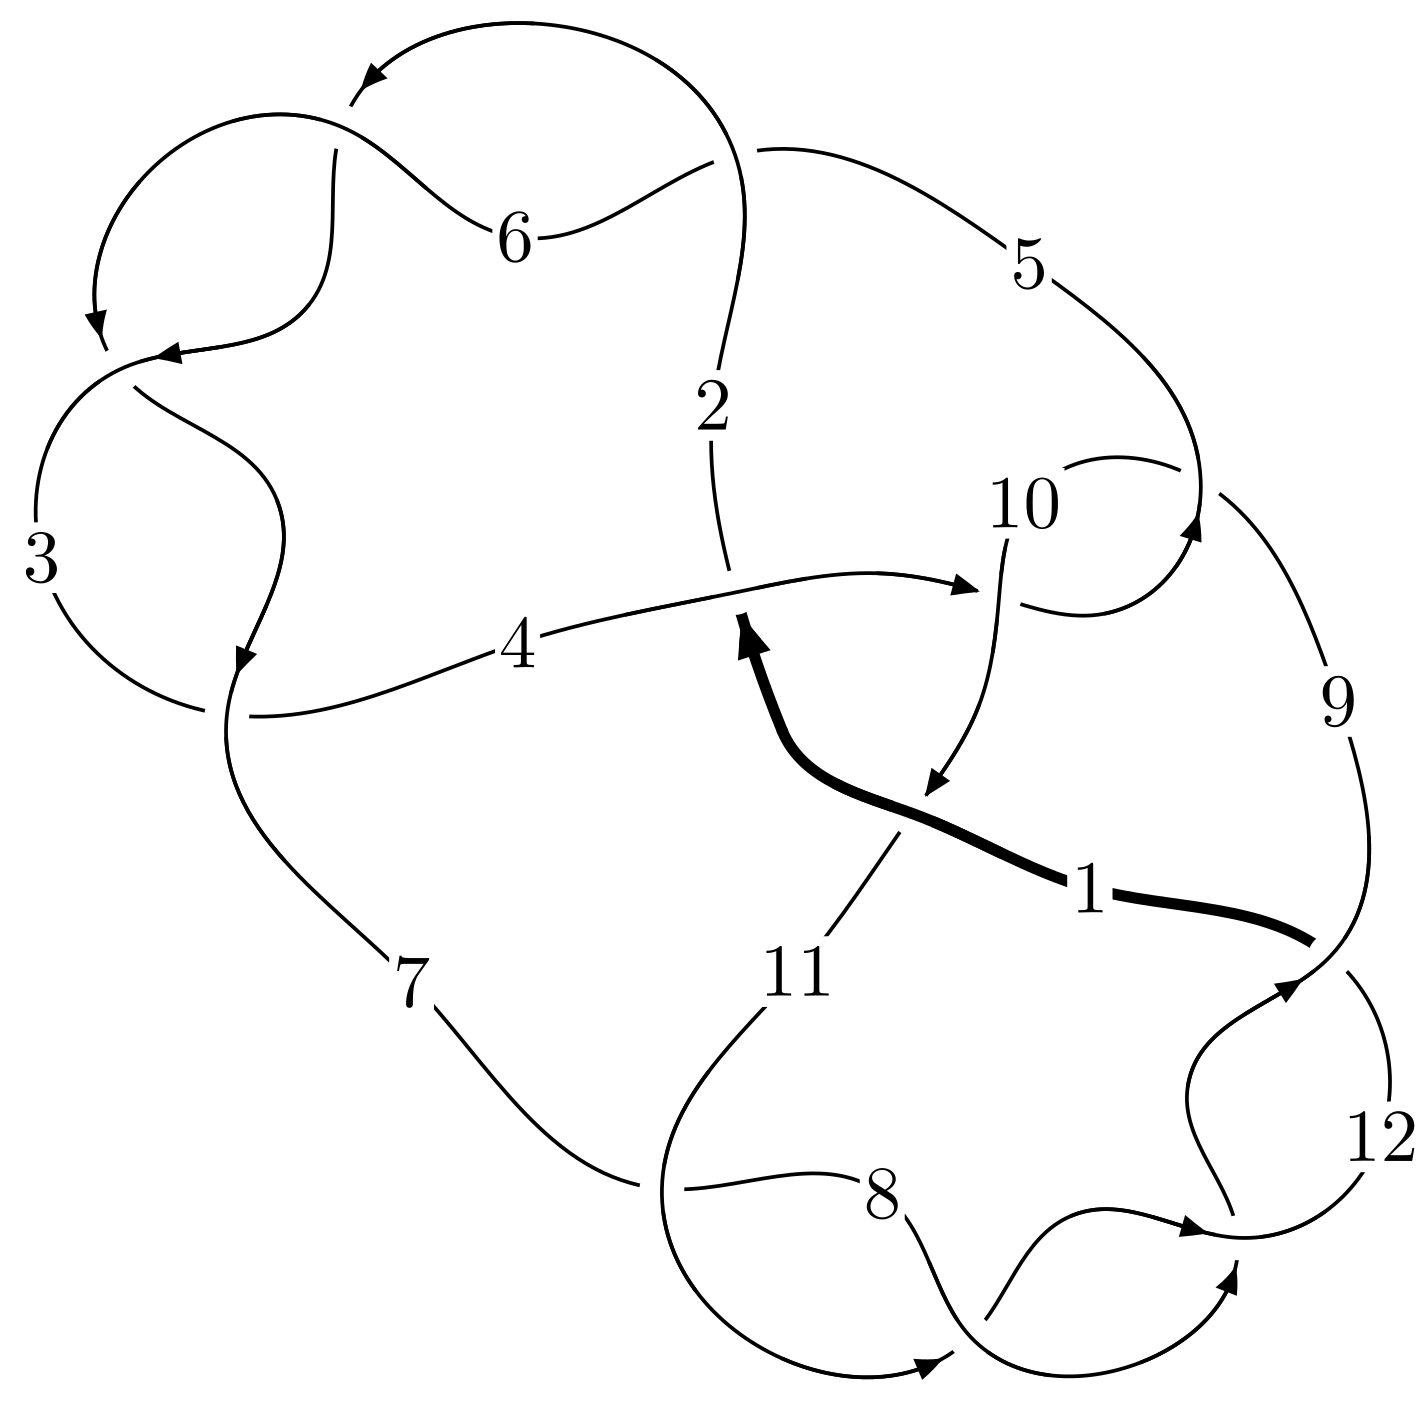
\includegraphics[width=112pt]{../../../GIT/diagram.site/Diagrams/png/1677_12a_0876.png}\\
\ \ \ A knot diagram\footnotemark}&
\allowdisplaybreaks
\textbf{Linearized knot diagam} \\
\cline{2-2}
 &
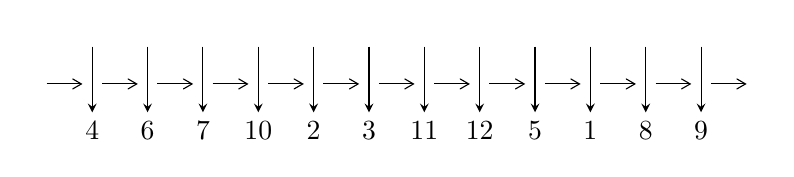
\begin{tikzpicture}[x=20pt, y=17pt]
	% nodes
	\node (C0) at (0, 0) {};
	\node (C1) at (1, 0) {};
	\node (C1U) at (1, +1) {};
	\node (C1D) at (1, -1) {4};

	\node (C2) at (2, 0) {};
	\node (C2U) at (2, +1) {};
	\node (C2D) at (2, -1) {6};

	\node (C3) at (3, 0) {};
	\node (C3U) at (3, +1) {};
	\node (C3D) at (3, -1) {7};

	\node (C4) at (4, 0) {};
	\node (C4U) at (4, +1) {};
	\node (C4D) at (4, -1) {10};

	\node (C5) at (5, 0) {};
	\node (C5U) at (5, +1) {};
	\node (C5D) at (5, -1) {2};

	\node (C6) at (6, 0) {};
	\node (C6U) at (6, +1) {};
	\node (C6D) at (6, -1) {3};

	\node (C7) at (7, 0) {};
	\node (C7U) at (7, +1) {};
	\node (C7D) at (7, -1) {11};

	\node (C8) at (8, 0) {};
	\node (C8U) at (8, +1) {};
	\node (C8D) at (8, -1) {12};

	\node (C9) at (9, 0) {};
	\node (C9U) at (9, +1) {};
	\node (C9D) at (9, -1) {5};

	\node (C10) at (10, 0) {};
	\node (C10U) at (10, +1) {};
	\node (C10D) at (10, -1) {1};

	\node (C11) at (11, 0) {};
	\node (C11U) at (11, +1) {};
	\node (C11D) at (11, -1) {8};

	\node (C12) at (12, 0) {};
	\node (C12U) at (12, +1) {};
	\node (C12D) at (12, -1) {9};
	\node (C13) at (13, 0) {};

	% arrows
	\draw[->,>={angle 60}]
	(C0) edge (C1) (C1) edge (C2) (C2) edge (C3) (C3) edge (C4) (C4) edge (C5) (C5) edge (C6) (C6) edge (C7) (C7) edge (C8) (C8) edge (C9) (C9) edge (C10) (C10) edge (C11) (C11) edge (C12) (C12) edge (C13) ;	\draw[->,>=stealth]
	(C1U) edge (C1D) (C2U) edge (C2D) (C3U) edge (C3D) (C4U) edge (C4D) (C5U) edge (C5D) (C6U) edge (C6D) (C7U) edge (C7D) (C8U) edge (C8D) (C9U) edge (C9D) (C10U) edge (C10D) (C11U) edge (C11D) (C12U) edge (C12D) ;
	\end{tikzpicture} \\
\hhline{~~} \\& 
\textbf{Solving Sequence} \\ \cline{2-2} 
 &
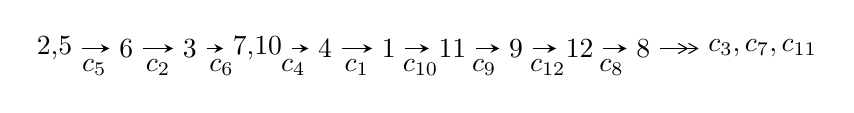
\begin{tikzpicture}[x=23pt, y=7pt]
	% node
	\node (A0) at (-1/8, 0) {2,5};
	\node (A1) at (1, 0) {6};
	\node (A2) at (2, 0) {3};
	\node (A3) at (49/16, 0) {7,10};
	\node (A4) at (33/8, 0) {4};
	\node (A5) at (41/8, 0) {1};
	\node (A6) at (49/8, 0) {11};
	\node (A7) at (57/8, 0) {9};
	\node (A8) at (65/8, 0) {12};
	\node (A9) at (73/8, 0) {8};
	\node (C1) at (1/2, -1) {$c_{5}$};
	\node (C2) at (3/2, -1) {$c_{2}$};
	\node (C3) at (5/2, -1) {$c_{6}$};
	\node (C4) at (29/8, -1) {$c_{4}$};
	\node (C5) at (37/8, -1) {$c_{1}$};
	\node (C6) at (45/8, -1) {$c_{10}$};
	\node (C7) at (53/8, -1) {$c_{9}$};
	\node (C8) at (61/8, -1) {$c_{12}$};
	\node (C9) at (69/8, -1) {$c_{8}$};
	\node (A10) at (11, 0) {$c_{3},c_{7},c_{11}$};

	% edge
	\draw[->,>=stealth]	
	(A0) edge (A1) (A1) edge (A2) (A2) edge (A3) (A3) edge (A4) (A4) edge (A5) (A5) edge (A6) (A6) edge (A7) (A7) edge (A8) (A8) edge (A9) ;
	\draw[->>,>={angle 60}]	
	(A9) edge (A10);
\end{tikzpicture} \\ 

\end{tabular} \\

\footnotetext{
The image of knot diagram is generated by the software ``\textbf{Draw programme}" developed by Andrew Bartholomew(\url{http://www.layer8.co.uk/maths/draw/index.htm\#Running-draw}), where we modified some parts for our purpose(\url{https://github.com/CATsTAILs/LinksPainter}).
}\phantom \\ \newline 
\centering \textbf{Ideals for irreducible components\footnotemark of $X_{\text{par}}$} 
 
\begin{align*}
I^u_{1}&=\langle 
u^{13}-8 u^{11}+23 u^9- u^8-28 u^7+5 u^6+14 u^5-7 u^4-4 u^3+2 u^2+b- u-1,\;- u^8+5 u^6-7 u^4+2 u^2+a-1,\\
\phantom{I^u_{1}}&\phantom{= \langle  }u^{14}+u^{13}-8 u^{12}-7 u^{11}+24 u^{10}+16 u^9-34 u^8-11 u^7+26 u^6-2 u^5-13 u^4+u^3+2 u^2-3 u-1\rangle \\
I^u_{2}&=\langle 
2 u^{41}+2 u^{40}+\cdots- u^2+b,\;-3 u^{41}-4 u^{40}+\cdots+a+1,\;u^{42}+2 u^{41}+\cdots+u+1\rangle \\
I^u_{3}&=\langle 
b,\;a+1,\;u^2- u-1\rangle \\
I^u_{4}&=\langle 
b,\;a+u-2,\;u^2- u-1\rangle \\
\\
\end{align*}
\raggedright * 4 irreducible components of $\dim_{\mathbb{C}}=0$, with total 60 representations.\\
\footnotetext{All coefficients of polynomials are rational numbers. But the coefficients are sometimes approximated in decimal forms when there is not enough margin.}
\newpage
\renewcommand{\arraystretch}{1}
\centering \section*{I. $I^u_{1}= \langle u^{13}-8 u^{11}+\cdots+b-1,\;- u^8+5 u^6-7 u^4+2 u^2+a-1,\;u^{14}+u^{13}+\cdots-3 u-1 \rangle$}
\flushleft \textbf{(i) Arc colorings}\\
\begin{tabular}{m{7pt} m{180pt} m{7pt} m{180pt} }
\flushright $a_{2}=$&$\begin{pmatrix}0\\u\end{pmatrix}$ \\
\flushright $a_{5}=$&$\begin{pmatrix}1\\0\end{pmatrix}$ \\
\flushright $a_{6}=$&$\begin{pmatrix}1\\u^2\end{pmatrix}$ \\
\flushright $a_{3}=$&$\begin{pmatrix}- u\\- u^3+u\end{pmatrix}$ \\
\flushright $a_{7}=$&$\begin{pmatrix}- u^2+1\\- u^4+2 u^2\end{pmatrix}$ \\
\flushright $a_{10}=$&$\begin{pmatrix}u^8-5 u^6+7 u^4-2 u^2+1\\- u^{13}+8 u^{11}+\cdots+u+1\end{pmatrix}$ \\
\flushright $a_{4}=$&$\begin{pmatrix}u^3-2 u\\u^5-3 u^3+u\end{pmatrix}$ \\
\flushright $a_{1}=$&$\begin{pmatrix}u^7-4 u^5+4 u^3\\u^9-5 u^7+7 u^5-2 u^3+u\end{pmatrix}$ \\
\flushright $a_{11}=$&$\begin{pmatrix}u^{11}-6 u^9+u^8+12 u^7-5 u^6-8 u^5+7 u^4-2 u^2+1\\u^{11}-6 u^9+u^8+12 u^7-5 u^6-9 u^5+7 u^4+2 u^3-2 u^2+u+1\end{pmatrix}$ \\
\flushright $a_{9}=$&$\begin{pmatrix}- u^{13}+8 u^{11}+\cdots+u+2\\- u^{13}+8 u^{11}+\cdots+u+1\end{pmatrix}$ \\
\flushright $a_{12}=$&$\begin{pmatrix}u^{13}-7 u^{11}+\cdots- u-1\\u^{13}-7 u^{11}+\cdots- u-1\end{pmatrix}$ \\
\flushright $a_{8}=$&$\begin{pmatrix}- u^{12}+6 u^{10}- u^9-12 u^8+5 u^7+8 u^6-7 u^5+2 u^3- u^2- u+1\\- u^{12}+6 u^{10}- u^9-12 u^8+5 u^7+9 u^6-7 u^5-3 u^4+2 u^3+u^2- u\end{pmatrix}$\\&\end{tabular}
\flushleft \textbf{(ii) Obstruction class $= -1$}\\~\\
\flushleft \textbf{(iii) Cusp Shapes $= -2 u^{13}+14 u^{11}-2 u^{10}-32 u^9+16 u^8+20 u^7-40 u^6+14 u^5+30 u^4-18 u^3+2 u^2+12 u-12$}\\~\\
\newpage\renewcommand{\arraystretch}{1}
\flushleft \textbf{(iv) u-Polynomials at the component}\newline \\
\begin{tabular}{m{50pt}|m{274pt}}
Crossings & \hspace{64pt}u-Polynomials at each crossing \\
\hline $$\begin{aligned}c_{1},c_{10}\end{aligned}$$&$\begin{aligned}
&u^{14}-3 u^{13}+\cdots-3 u-1
\end{aligned}$\\
\hline $$\begin{aligned}c_{2},c_{3},c_{5}\\c_{6},c_{7},c_{8}\\c_{11},c_{12}\end{aligned}$$&$\begin{aligned}
&u^{14}+u^{13}+\cdots-3 u-1
\end{aligned}$\\
\hline $$\begin{aligned}c_{4},c_{9}\end{aligned}$$&$\begin{aligned}
&u^{14}-5 u^{13}+\cdots-8 u+4
\end{aligned}$\\
\hline
\end{tabular}\\~\\
\newpage\renewcommand{\arraystretch}{1}
\flushleft \textbf{(v) Riley Polynomials at the component}\newline \\
\begin{tabular}{m{50pt}|m{274pt}}
Crossings & \hspace{64pt}Riley Polynomials at each crossing \\
\hline $$\begin{aligned}c_{1},c_{10}\end{aligned}$$&$\begin{aligned}
&y^{14}+7 y^{13}+\cdots-29 y+1
\end{aligned}$\\
\hline $$\begin{aligned}c_{2},c_{3},c_{5}\\c_{6},c_{7},c_{8}\\c_{11},c_{12}\end{aligned}$$&$\begin{aligned}
&y^{14}-17 y^{13}+\cdots-13 y+1
\end{aligned}$\\
\hline $$\begin{aligned}c_{4},c_{9}\end{aligned}$$&$\begin{aligned}
&y^{14}+5 y^{13}+\cdots-64 y+16
\end{aligned}$\\
\hline
\end{tabular}\\~\\
\newpage\flushleft \textbf{(vi) Complex Volumes and Cusp Shapes}
$$\begin{array}{c|c|c}  
\text{Solutions to }I^u_{1}& \I (\text{vol} + \sqrt{-1}CS) & \text{Cusp shape}\\
 \hline 
\begin{aligned}
u &= \phantom{-}0.680303 + 0.531876 I \\
a &= -1.24132 + 1.66316 I \\
b &= -0.572300 - 1.150040 I\end{aligned}
 & \phantom{-}1.04590 - 7.72861 I & -13.6329 + 9.6019 I \\ \hline\begin{aligned}
u &= \phantom{-}0.680303 - 0.531876 I \\
a &= -1.24132 - 1.66316 I \\
b &= -0.572300 + 1.150040 I\end{aligned}
 & \phantom{-}1.04590 + 7.72861 I & -13.6329 - 9.6019 I \\ \hline\begin{aligned}
u &= -0.593521 + 0.378079 I \\
a &= \phantom{-}0.054243 - 0.515402 I \\
b &= -0.834976 - 0.363198 I\end{aligned}
 & -1.38750 + 2.49320 I & -16.0799 - 7.8719 I \\ \hline\begin{aligned}
u &= -0.593521 - 0.378079 I \\
a &= \phantom{-}0.054243 + 0.515402 I \\
b &= -0.834976 + 0.363198 I\end{aligned}
 & -1.38750 - 2.49320 I & -16.0799 + 7.8719 I \\ \hline\begin{aligned}
u &= \phantom{-}0.303532 + 0.566158 I \\
a &= \phantom{-}0.62968 - 1.83164 I \\
b &= -0.251015 + 1.107770 I\end{aligned}
 & \phantom{-}3.30391 + 0.11980 I & -7.23583 + 2.81079 I \\ \hline\begin{aligned}
u &= \phantom{-}0.303532 - 0.566158 I \\
a &= \phantom{-}0.62968 + 1.83164 I \\
b &= -0.251015 - 1.107770 I\end{aligned}
 & \phantom{-}3.30391 - 0.11980 I & -7.23583 - 2.81079 I \\ \hline\begin{aligned}
u &= -1.45549 + 0.12558 I \\
a &= \phantom{-}0.560799 + 0.786391 I \\
b &= \phantom{-}0.204002 - 1.257830 I\end{aligned}
 & -8.06473 + 4.40167 I & -16.0274 - 3.4872 I \\ \hline\begin{aligned}
u &= -1.45549 - 0.12558 I \\
a &= \phantom{-}0.560799 - 0.786391 I \\
b &= \phantom{-}0.204002 + 1.257830 I\end{aligned}
 & -8.06473 - 4.40167 I & -16.0274 + 3.4872 I \\ \hline\begin{aligned}
u &= \phantom{-}1.48768\phantom{ +0.000000I} \\
a &= \phantom{-}0.650213\phantom{ +0.000000I} \\
b &= \phantom{-}1.05020\phantom{ +0.000000I}\end{aligned}
 & -12.8678\phantom{ +0.000000I} & -19.3260\phantom{ +0.000000I} \\ \hline\begin{aligned}
u &= \phantom{-}1.58880 + 0.12925 I \\
a &= -0.470390 + 0.414195 I \\
b &= -1.052550 + 0.599886 I\end{aligned}
 & -16.3668 - 6.3822 I & -20.6641 + 3.1830 I\\
 \hline 
 \end{array}$$\newpage$$\begin{array}{c|c|c}  
\text{Solutions to }I^u_{1}& \I (\text{vol} + \sqrt{-1}CS) & \text{Cusp shape}\\
 \hline 
\begin{aligned}
u &= \phantom{-}1.58880 - 0.12925 I \\
a &= -0.470390 - 0.414195 I \\
b &= -1.052550 - 0.599886 I\end{aligned}
 & -16.3668 + 6.3822 I & -20.6641 - 3.1830 I \\ \hline\begin{aligned}
u &= -1.61264 + 0.16202 I \\
a &= -1.29225 - 0.74678 I \\
b &= -0.754602 + 1.160230 I\end{aligned}
 & -14.5457 + 12.9375 I & -19.3006 - 6.7062 I \\ \hline\begin{aligned}
u &= -1.61264 - 0.16202 I \\
a &= -1.29225 + 0.74678 I \\
b &= -0.754602 - 1.160230 I\end{aligned}
 & -14.5457 - 12.9375 I & -19.3006 + 6.7062 I \\ \hline\begin{aligned}
u &= -0.309637\phantom{ +0.000000I} \\
a &= \phantom{-}0.868272\phantom{ +0.000000I} \\
b &= \phantom{-}0.472677\phantom{ +0.000000I}\end{aligned}
 & -0.638892\phantom{ +0.000000I} & -14.7920\phantom{ +0.000000I}\\
 \hline 
 \end{array}$$\newpage\newpage\renewcommand{\arraystretch}{1}
\centering \section*{II. $I^u_{2}= \langle 2 u^{41}+2 u^{40}+\cdots- u^2+b,\;-3 u^{41}-4 u^{40}+\cdots+a+1,\;u^{42}+2 u^{41}+\cdots+u+1 \rangle$}
\flushleft \textbf{(i) Arc colorings}\\
\begin{tabular}{m{7pt} m{180pt} m{7pt} m{180pt} }
\flushright $a_{2}=$&$\begin{pmatrix}0\\u\end{pmatrix}$ \\
\flushright $a_{5}=$&$\begin{pmatrix}1\\0\end{pmatrix}$ \\
\flushright $a_{6}=$&$\begin{pmatrix}1\\u^2\end{pmatrix}$ \\
\flushright $a_{3}=$&$\begin{pmatrix}- u\\- u^3+u\end{pmatrix}$ \\
\flushright $a_{7}=$&$\begin{pmatrix}- u^2+1\\- u^4+2 u^2\end{pmatrix}$ \\
\flushright $a_{10}=$&$\begin{pmatrix}3 u^{41}+4 u^{40}+\cdots-6 u-1\\-2 u^{41}-2 u^{40}+\cdots-6 u^3+u^2\end{pmatrix}$ \\
\flushright $a_{4}=$&$\begin{pmatrix}u^3-2 u\\u^5-3 u^3+u\end{pmatrix}$ \\
\flushright $a_{1}=$&$\begin{pmatrix}u^7-4 u^5+4 u^3\\u^9-5 u^7+7 u^5-2 u^3+u\end{pmatrix}$ \\
\flushright $a_{11}=$&$\begin{pmatrix}u^{40}- u^{39}+\cdots-5 u-1\\-3 u^{41}-3 u^{40}+\cdots-5 u^3+2 u^2\end{pmatrix}$ \\
\flushright $a_{9}=$&$\begin{pmatrix}u^{41}+2 u^{40}+\cdots-6 u-1\\-2 u^{41}-2 u^{40}+\cdots-6 u^3+u^2\end{pmatrix}$ \\
\flushright $a_{12}=$&$\begin{pmatrix}- u^{41}-2 u^{40}+\cdots-2 u^2+u\\- u^{14}+8 u^{12}+\cdots+u^2+2 u\end{pmatrix}$ \\
\flushright $a_{8}=$&$\begin{pmatrix}2 u^{41}+3 u^{40}+\cdots- u+1\\u^{41}+u^{40}+\cdots+7 u^3-2 u\end{pmatrix}$\\&\end{tabular}
\flushleft \textbf{(ii) Obstruction class $= -1$}\\~\\
\flushleft \textbf{(iii) Cusp Shapes $= 3 u^{40}+3 u^{39}+\cdots+18 u^2-15$}\\~\\
\newpage\renewcommand{\arraystretch}{1}
\flushleft \textbf{(iv) u-Polynomials at the component}\newline \\
\begin{tabular}{m{50pt}|m{274pt}}
Crossings & \hspace{64pt}u-Polynomials at each crossing \\
\hline $$\begin{aligned}c_{1},c_{10}\end{aligned}$$&$\begin{aligned}
&u^{42}-12 u^{41}+\cdots+53 u+31
\end{aligned}$\\
\hline $$\begin{aligned}c_{2},c_{3},c_{5}\\c_{6},c_{7},c_{8}\\c_{11},c_{12}\end{aligned}$$&$\begin{aligned}
&u^{42}+2 u^{41}+\cdots+u+1
\end{aligned}$\\
\hline $$\begin{aligned}c_{4},c_{9}\end{aligned}$$&$\begin{aligned}
&(u^{21}+2 u^{20}+\cdots+5 u+2)^{2}
\end{aligned}$\\
\hline
\end{tabular}\\~\\
\newpage\renewcommand{\arraystretch}{1}
\flushleft \textbf{(v) Riley Polynomials at the component}\newline \\
\begin{tabular}{m{50pt}|m{274pt}}
Crossings & \hspace{64pt}Riley Polynomials at each crossing \\
\hline $$\begin{aligned}c_{1},c_{10}\end{aligned}$$&$\begin{aligned}
&y^{42}-12 y^{41}+\cdots+34825 y+961
\end{aligned}$\\
\hline $$\begin{aligned}c_{2},c_{3},c_{5}\\c_{6},c_{7},c_{8}\\c_{11},c_{12}\end{aligned}$$&$\begin{aligned}
&y^{42}-48 y^{41}+\cdots-11 y+1
\end{aligned}$\\
\hline $$\begin{aligned}c_{4},c_{9}\end{aligned}$$&$\begin{aligned}
&(y^{21}+10 y^{20}+\cdots-15 y-4)^{2}
\end{aligned}$\\
\hline
\end{tabular}\\~\\
\newpage\flushleft \textbf{(vi) Complex Volumes and Cusp Shapes}
$$\begin{array}{c|c|c}  
\text{Solutions to }I^u_{2}& \I (\text{vol} + \sqrt{-1}CS) & \text{Cusp shape}\\
 \hline 
\begin{aligned}
u &= -0.952260 + 0.275050 I \\
a &= -0.237674 + 0.141836 I \\
b &= \phantom{-}0.469429 + 1.026280 I\end{aligned}
 & -8.66083 - 3.12379 I & -18.1716 + 1.7818 I \\ \hline\begin{aligned}
u &= -0.952260 - 0.275050 I \\
a &= -0.237674 - 0.141836 I \\
b &= \phantom{-}0.469429 - 1.026280 I\end{aligned}
 & -8.66083 + 3.12379 I & -18.1716 - 1.7818 I \\ \hline\begin{aligned}
u &= -0.892649 + 0.147229 I \\
a &= \phantom{-}0.102532 - 0.122821 I \\
b &= -0.268462 - 0.851142 I\end{aligned}
 & -1.46292 - 1.33471 I & -14.9864 + 4.7477 I \\ \hline\begin{aligned}
u &= -0.892649 - 0.147229 I \\
a &= \phantom{-}0.102532 + 0.122821 I \\
b &= -0.268462 + 0.851142 I\end{aligned}
 & -1.46292 + 1.33471 I & -14.9864 - 4.7477 I \\ \hline\begin{aligned}
u &= \phantom{-}0.723689 + 0.540993 I \\
a &= \phantom{-}1.26266 - 1.59018 I \\
b &= \phantom{-}0.677487 + 1.162350 I\end{aligned}
 & -6.63828 - 10.29320 I & -16.6887 + 8.0442 I \\ \hline\begin{aligned}
u &= \phantom{-}0.723689 - 0.540993 I \\
a &= \phantom{-}1.26266 + 1.59018 I \\
b &= \phantom{-}0.677487 - 1.162350 I\end{aligned}
 & -6.63828 + 10.29320 I & -16.6887 - 8.0442 I \\ \hline\begin{aligned}
u &= \phantom{-}0.622201 + 0.517014 I \\
a &= \phantom{-}1.19658 - 1.76438 I \\
b &= \phantom{-}0.436892 + 1.122040 I\end{aligned}
 & \phantom{-}2.37193 - 3.84440 I & -10.04174 + 4.38533 I \\ \hline\begin{aligned}
u &= \phantom{-}0.622201 - 0.517014 I \\
a &= \phantom{-}1.19658 + 1.76438 I \\
b &= \phantom{-}0.436892 - 1.122040 I\end{aligned}
 & \phantom{-}2.37193 + 3.84440 I & -10.04174 - 4.38533 I \\ \hline\begin{aligned}
u &= -0.650081 + 0.454963 I \\
a &= -0.175433 + 0.522705 I \\
b &= \phantom{-}0.982337 + 0.491258 I\end{aligned}
 & -8.77344 + 4.23823 I & -18.3836 - 4.9951 I \\ \hline\begin{aligned}
u &= -0.650081 - 0.454963 I \\
a &= -0.175433 - 0.522705 I \\
b &= \phantom{-}0.982337 - 0.491258 I\end{aligned}
 & -8.77344 - 4.23823 I & -18.3836 + 4.9951 I\\
 \hline 
 \end{array}$$\newpage$$\begin{array}{c|c|c}  
\text{Solutions to }I^u_{2}& \I (\text{vol} + \sqrt{-1}CS) & \text{Cusp shape}\\
 \hline 
\begin{aligned}
u &= \phantom{-}0.452901 + 0.570594 I \\
a &= -0.88626 + 1.82784 I \\
b &= -0.052121 - 1.208570 I\end{aligned}
 & -1.92244 - 1.93968 I & -12.20153 + 3.66263 I \\ \hline\begin{aligned}
u &= \phantom{-}0.452901 - 0.570594 I \\
a &= -0.88626 - 1.82784 I \\
b &= -0.052121 + 1.208570 I\end{aligned}
 & -1.92244 + 1.93968 I & -12.20153 - 3.66263 I \\ \hline\begin{aligned}
u &= \phantom{-}0.631403 + 0.254962 I \\
a &= \phantom{-}1.91563 - 2.30921 I \\
b &= \phantom{-}0.397322 + 0.594617 I\end{aligned}
 & -10.10480 - 0.64503 I & -18.1436 + 8.7498 I \\ \hline\begin{aligned}
u &= \phantom{-}0.631403 - 0.254962 I \\
a &= \phantom{-}1.91563 + 2.30921 I \\
b &= \phantom{-}0.397322 - 0.594617 I\end{aligned}
 & -10.10480 + 0.64503 I & -18.1436 - 8.7498 I \\ \hline\begin{aligned}
u &= \phantom{-}0.178370 + 0.653047 I \\
a &= \phantom{-}0.50210 - 1.62752 I \\
b &= -0.580700 + 1.149510 I\end{aligned}
 & -5.02807 + 6.26735 I & -13.39857 - 3.31929 I \\ \hline\begin{aligned}
u &= \phantom{-}0.178370 - 0.653047 I \\
a &= \phantom{-}0.50210 + 1.62752 I \\
b &= -0.580700 - 1.149510 I\end{aligned}
 & -5.02807 - 6.26735 I & -13.39857 + 3.31929 I \\ \hline\begin{aligned}
u &= \phantom{-}0.543160 + 0.383707 I \\
a &= -1.24755 + 2.15130 I \\
b &= -0.268462 - 0.851142 I\end{aligned}
 & -1.46292 - 1.33471 I & -14.9864 + 4.7477 I \\ \hline\begin{aligned}
u &= \phantom{-}0.543160 - 0.383707 I \\
a &= -1.24755 - 2.15130 I \\
b &= -0.268462 + 0.851142 I\end{aligned}
 & -1.46292 + 1.33471 I & -14.9864 - 4.7477 I \\ \hline\begin{aligned}
u &= \phantom{-}0.227652 + 0.609745 I \\
a &= -0.53434 + 1.72086 I \\
b &= \phantom{-}0.436892 - 1.122040 I\end{aligned}
 & \phantom{-}2.37193 + 3.84440 I & -10.04174 - 4.38533 I \\ \hline\begin{aligned}
u &= \phantom{-}0.227652 - 0.609745 I \\
a &= -0.53434 - 1.72086 I \\
b &= \phantom{-}0.436892 + 1.122040 I\end{aligned}
 & \phantom{-}2.37193 - 3.84440 I & -10.04174 + 4.38533 I\\
 \hline 
 \end{array}$$\newpage$$\begin{array}{c|c|c}  
\text{Solutions to }I^u_{2}& \I (\text{vol} + \sqrt{-1}CS) & \text{Cusp shape}\\
 \hline 
\begin{aligned}
u &= -1.409680 + 0.044575 I \\
a &= -0.180441 - 0.797743 I \\
b &= -0.052121 + 1.208570 I\end{aligned}
 & -1.92244 + 1.93968 I & \phantom{-0.000000 } 0 \\ \hline\begin{aligned}
u &= -1.409680 - 0.044575 I \\
a &= -0.180441 + 0.797743 I \\
b &= -0.052121 - 1.208570 I\end{aligned}
 & -1.92244 - 1.93968 I & \phantom{-0.000000 } 0 \\ \hline\begin{aligned}
u &= -0.226402 + 0.475799 I \\
a &= -0.056046 - 1.133970 I \\
b &= -0.885131 + 0.313438 I\end{aligned}
 & -7.56038 - 0.95789 I & -15.2596 - 1.5508 I \\ \hline\begin{aligned}
u &= -0.226402 - 0.475799 I \\
a &= -0.056046 + 1.133970 I \\
b &= -0.885131 - 0.313438 I\end{aligned}
 & -7.56038 + 0.95789 I & -15.2596 + 1.5508 I \\ \hline\begin{aligned}
u &= \phantom{-}1.56042 + 0.06421 I \\
a &= -0.462955 + 0.220565 I \\
b &= -0.885131 + 0.313438 I\end{aligned}
 & -7.56038 - 0.95789 I & \phantom{-0.000000 } 0 \\ \hline\begin{aligned}
u &= \phantom{-}1.56042 - 0.06421 I \\
a &= -0.462955 - 0.220565 I \\
b &= -0.885131 - 0.313438 I\end{aligned}
 & -7.56038 + 0.95789 I & \phantom{-0.000000 } 0 \\ \hline\begin{aligned}
u &= -1.56589 + 0.11035 I \\
a &= \phantom{-}1.08354 + 1.11273 I \\
b &= \phantom{-}0.469429 - 1.026280 I\end{aligned}
 & -8.66083 + 3.12379 I & \phantom{-0.000000 } 0 \\ \hline\begin{aligned}
u &= -1.56589 - 0.11035 I \\
a &= \phantom{-}1.08354 - 1.11273 I \\
b &= \phantom{-}0.469429 + 1.026280 I\end{aligned}
 & -8.66083 - 3.12379 I & \phantom{-0.000000 } 0 \\ \hline\begin{aligned}
u &= \phantom{-}1.57529 + 0.10471 I \\
a &= \phantom{-}0.470499 - 0.343906 I \\
b &= \phantom{-}0.982337 - 0.491258 I\end{aligned}
 & -8.77344 - 4.23823 I & \phantom{-0.000000 } 0 \\ \hline\begin{aligned}
u &= \phantom{-}1.57529 - 0.10471 I \\
a &= \phantom{-}0.470499 + 0.343906 I \\
b &= \phantom{-}0.982337 + 0.491258 I\end{aligned}
 & -8.77344 + 4.23823 I & \phantom{-0.000000 } 0\\
 \hline 
 \end{array}$$\newpage$$\begin{array}{c|c|c}  
\text{Solutions to }I^u_{2}& \I (\text{vol} + \sqrt{-1}CS) & \text{Cusp shape}\\
 \hline 
\begin{aligned}
u &= -0.359452 + 0.212787 I \\
a &= \phantom{-}0.467612 + 0.591791 I \\
b &= \phantom{-}0.596034\phantom{ +0.000000I}\end{aligned}
 & -0.606975\phantom{ +0.000000I} & -13.01685 + 0. I\phantom{ +0.000000I} \\ \hline\begin{aligned}
u &= -0.359452 - 0.212787 I \\
a &= \phantom{-}0.467612 - 0.591791 I \\
b &= \phantom{-}0.596034\phantom{ +0.000000I}\end{aligned}
 & -0.606975\phantom{ +0.000000I} & -13.01685 + 0. I\phantom{ +0.000000I} \\ \hline\begin{aligned}
u &= -1.57630 + 0.14785 I \\
a &= -1.13809 - 0.86977 I \\
b &= -0.580700 + 1.149510 I\end{aligned}
 & -5.02807 + 6.26735 I & \phantom{-0.000000 } 0 \\ \hline\begin{aligned}
u &= -1.57630 - 0.14785 I \\
a &= -1.13809 + 0.86977 I \\
b &= -0.580700 - 1.149510 I\end{aligned}
 & -5.02807 - 6.26735 I & \phantom{-0.000000 } 0 \\ \hline\begin{aligned}
u &= -1.58753 + 0.08171 I \\
a &= -1.29868 - 1.37872 I \\
b &= -0.475070 + 0.853809 I\end{aligned}
 & -17.7147 + 1.9468 I & \phantom{-0.000000 } 0 \\ \hline\begin{aligned}
u &= -1.58753 - 0.08171 I \\
a &= -1.29868 + 1.37872 I \\
b &= -0.475070 - 0.853809 I\end{aligned}
 & -17.7147 - 1.9468 I & \phantom{-0.000000 } 0 \\ \hline\begin{aligned}
u &= -1.59635 + 0.15789 I \\
a &= \phantom{-}1.22706 + 0.79548 I \\
b &= \phantom{-}0.677487 - 1.162350 I\end{aligned}
 & -6.63828 + 10.29320 I & \phantom{-0.000000 } 0 \\ \hline\begin{aligned}
u &= -1.59635 - 0.15789 I \\
a &= \phantom{-}1.22706 - 0.79548 I \\
b &= \phantom{-}0.677487 + 1.162350 I\end{aligned}
 & -6.63828 - 10.29320 I & \phantom{-0.000000 } 0 \\ \hline\begin{aligned}
u &= \phantom{-}1.63726 + 0.03700 I \\
a &= \phantom{-}0.176213 - 0.298794 I \\
b &= \phantom{-}0.397322 - 0.594617 I\end{aligned}
 & -10.10480 + 0.64503 I & \phantom{-0.000000 } 0 \\ \hline\begin{aligned}
u &= \phantom{-}1.63726 - 0.03700 I \\
a &= \phantom{-}0.176213 + 0.298794 I \\
b &= \phantom{-}0.397322 + 0.594617 I\end{aligned}
 & -10.10480 - 0.64503 I & \phantom{-0.000000 } 0\\
 \hline 
 \end{array}$$\newpage$$\begin{array}{c|c|c}  
\text{Solutions to }I^u_{2}& \I (\text{vol} + \sqrt{-1}CS) & \text{Cusp shape}\\
 \hline 
\begin{aligned}
u &= \phantom{-}1.66424 + 0.05653 I \\
a &= -0.186954 + 0.414396 I \\
b &= -0.475070 + 0.853809 I\end{aligned}
 & -17.7147 + 1.9468 I & \phantom{-0.000000 } 0 \\ \hline\begin{aligned}
u &= \phantom{-}1.66424 - 0.05653 I \\
a &= -0.186954 - 0.414396 I \\
b &= -0.475070 - 0.853809 I\end{aligned}
 & -17.7147 - 1.9468 I & \phantom{-0.000000 } 0\\
 \hline 
 \end{array}$$\newpage\newpage\renewcommand{\arraystretch}{1}
\centering \section*{III. $I^u_{3}= \langle b,\;a+1,\;u^2- u-1 \rangle$}
\flushleft \textbf{(i) Arc colorings}\\
\begin{tabular}{m{7pt} m{180pt} m{7pt} m{180pt} }
\flushright $a_{2}=$&$\begin{pmatrix}0\\u\end{pmatrix}$ \\
\flushright $a_{5}=$&$\begin{pmatrix}1\\0\end{pmatrix}$ \\
\flushright $a_{6}=$&$\begin{pmatrix}1\\u+1\end{pmatrix}$ \\
\flushright $a_{3}=$&$\begin{pmatrix}- u\\- u-1\end{pmatrix}$ \\
\flushright $a_{7}=$&$\begin{pmatrix}- u\\- u\end{pmatrix}$ \\
\flushright $a_{10}=$&$\begin{pmatrix}-1\\0\end{pmatrix}$ \\
\flushright $a_{4}=$&$\begin{pmatrix}1\\0\end{pmatrix}$ \\
\flushright $a_{1}=$&$\begin{pmatrix}u\\u\end{pmatrix}$ \\
\flushright $a_{11}=$&$\begin{pmatrix}- u-2\\- u-1\end{pmatrix}$ \\
\flushright $a_{9}=$&$\begin{pmatrix}-1\\0\end{pmatrix}$ \\
\flushright $a_{12}=$&$\begin{pmatrix}2 u\\u\end{pmatrix}$ \\
\flushright $a_{8}=$&$\begin{pmatrix}2 u+1\\u+1\end{pmatrix}$\\&\end{tabular}
\flushleft \textbf{(ii) Obstruction class $= 1$}\\~\\
\flushleft \textbf{(iii) Cusp Shapes $= -20$}\\~\\
\newpage\renewcommand{\arraystretch}{1}
\flushleft \textbf{(iv) u-Polynomials at the component}\newline \\
\begin{tabular}{m{50pt}|m{274pt}}
Crossings & \hspace{64pt}u-Polynomials at each crossing \\
\hline $$\begin{aligned}c_{1},c_{2},c_{3}\\c_{7},c_{8},c_{10}\end{aligned}$$&$\begin{aligned}
&u^2+u-1
\end{aligned}$\\
\hline $$\begin{aligned}c_{4},c_{9}\end{aligned}$$&$\begin{aligned}
&u^2
\end{aligned}$\\
\hline $$\begin{aligned}c_{5},c_{6},c_{11}\\c_{12}\end{aligned}$$&$\begin{aligned}
&u^2- u-1
\end{aligned}$\\
\hline
\end{tabular}\\~\\
\newpage\renewcommand{\arraystretch}{1}
\flushleft \textbf{(v) Riley Polynomials at the component}\newline \\
\begin{tabular}{m{50pt}|m{274pt}}
Crossings & \hspace{64pt}Riley Polynomials at each crossing \\
\hline $$\begin{aligned}c_{1},c_{2},c_{3}\\c_{5},c_{6},c_{7}\\c_{8},c_{10},c_{11}\\c_{12}\end{aligned}$$&$\begin{aligned}
&y^2-3 y+1
\end{aligned}$\\
\hline $$\begin{aligned}c_{4},c_{9}\end{aligned}$$&$\begin{aligned}
&y^2
\end{aligned}$\\
\hline
\end{tabular}\\~\\
\newpage\flushleft \textbf{(vi) Complex Volumes and Cusp Shapes}
$$\begin{array}{c|c|c}  
\text{Solutions to }I^u_{3}& \I (\text{vol} + \sqrt{-1}CS) & \text{Cusp shape}\\
 \hline 
\begin{aligned}
u &= -0.618034\phantom{ +0.000000I} \\
a &= -1.00000\phantom{ +0.000000I} \\
b &= \phantom{-0.000000 } 0\end{aligned}
 & -1.97392\phantom{ +0.000000I} & -20.0000\phantom{ +0.000000I} \\ \hline\begin{aligned}
u &= \phantom{-}1.61803\phantom{ +0.000000I} \\
a &= -1.00000\phantom{ +0.000000I} \\
b &= \phantom{-0.000000 } 0\end{aligned}
 & -17.7653\phantom{ +0.000000I} & -20.0000\phantom{ +0.000000I}\\
 \hline 
 \end{array}$$\newpage\newpage\renewcommand{\arraystretch}{1}
\centering \section*{IV. $I^u_{4}= \langle b,\;a+u-2,\;u^2- u-1 \rangle$}
\flushleft \textbf{(i) Arc colorings}\\
\begin{tabular}{m{7pt} m{180pt} m{7pt} m{180pt} }
\flushright $a_{2}=$&$\begin{pmatrix}0\\u\end{pmatrix}$ \\
\flushright $a_{5}=$&$\begin{pmatrix}1\\0\end{pmatrix}$ \\
\flushright $a_{6}=$&$\begin{pmatrix}1\\u+1\end{pmatrix}$ \\
\flushright $a_{3}=$&$\begin{pmatrix}- u\\- u-1\end{pmatrix}$ \\
\flushright $a_{7}=$&$\begin{pmatrix}- u\\- u\end{pmatrix}$ \\
\flushright $a_{10}=$&$\begin{pmatrix}- u+2\\0\end{pmatrix}$ \\
\flushright $a_{4}=$&$\begin{pmatrix}1\\0\end{pmatrix}$ \\
\flushright $a_{1}=$&$\begin{pmatrix}u\\u\end{pmatrix}$ \\
\flushright $a_{11}=$&$\begin{pmatrix}- u+3\\1\end{pmatrix}$ \\
\flushright $a_{9}=$&$\begin{pmatrix}- u+2\\0\end{pmatrix}$ \\
\flushright $a_{12}=$&$\begin{pmatrix}3 u-3\\u\end{pmatrix}$ \\
\flushright $a_{8}=$&$\begin{pmatrix}2 u-4\\-1\end{pmatrix}$\\&\end{tabular}
\flushleft \textbf{(ii) Obstruction class $= 1$}\\~\\
\flushleft \textbf{(iii) Cusp Shapes $= -15$}\\~\\
\newpage\renewcommand{\arraystretch}{1}
\flushleft \textbf{(iv) u-Polynomials at the component}\newline \\
\begin{tabular}{m{50pt}|m{274pt}}
Crossings & \hspace{64pt}u-Polynomials at each crossing \\
\hline $$\begin{aligned}c_{1},c_{2},c_{3}\\c_{7},c_{8},c_{10}\end{aligned}$$&$\begin{aligned}
&u^2+u-1
\end{aligned}$\\
\hline $$\begin{aligned}c_{4},c_{9}\end{aligned}$$&$\begin{aligned}
&u^2
\end{aligned}$\\
\hline $$\begin{aligned}c_{5},c_{6},c_{11}\\c_{12}\end{aligned}$$&$\begin{aligned}
&u^2- u-1
\end{aligned}$\\
\hline
\end{tabular}\\~\\
\newpage\renewcommand{\arraystretch}{1}
\flushleft \textbf{(v) Riley Polynomials at the component}\newline \\
\begin{tabular}{m{50pt}|m{274pt}}
Crossings & \hspace{64pt}Riley Polynomials at each crossing \\
\hline $$\begin{aligned}c_{1},c_{2},c_{3}\\c_{5},c_{6},c_{7}\\c_{8},c_{10},c_{11}\\c_{12}\end{aligned}$$&$\begin{aligned}
&y^2-3 y+1
\end{aligned}$\\
\hline $$\begin{aligned}c_{4},c_{9}\end{aligned}$$&$\begin{aligned}
&y^2
\end{aligned}$\\
\hline
\end{tabular}\\~\\
\newpage\flushleft \textbf{(vi) Complex Volumes and Cusp Shapes}
$$\begin{array}{c|c|c}  
\text{Solutions to }I^u_{4}& \I (\text{vol} + \sqrt{-1}CS) & \text{Cusp shape}\\
 \hline 
\begin{aligned}
u &= -0.618034\phantom{ +0.000000I} \\
a &= \phantom{-}2.61803\phantom{ +0.000000I} \\
b &= \phantom{-0.000000 } 0\end{aligned}
 & -9.86960\phantom{ +0.000000I} & -15.0000\phantom{ +0.000000I} \\ \hline\begin{aligned}
u &= \phantom{-}1.61803\phantom{ +0.000000I} \\
a &= \phantom{-}0.381966\phantom{ +0.000000I} \\
b &= \phantom{-0.000000 } 0\end{aligned}
 & -9.86960\phantom{ +0.000000I} & -15.0000\phantom{ +0.000000I}\\
 \hline 
 \end{array}$$\newpage
\newpage\renewcommand{\arraystretch}{1}
\centering \section*{ V. u-Polynomials}
\begin{tabular}{m{50pt}|m{274pt}}
Crossings & \hspace{64pt}u-Polynomials at each crossing \\
\hline $$\begin{aligned}c_{1},c_{10}\end{aligned}$$&$\begin{aligned}
&((u^2+u-1)^2)(u^{14}-3 u^{13}+\cdots-3 u-1)(u^{42}-12 u^{41}+\cdots+53 u+31)
\end{aligned}$\\
\hline $$\begin{aligned}c_{2},c_{3},c_{7}\\c_{8}\end{aligned}$$&$\begin{aligned}
&((u^2+u-1)^2)(u^{14}+u^{13}+\cdots-3 u-1)(u^{42}+2 u^{41}+\cdots+u+1)
\end{aligned}$\\
\hline $$\begin{aligned}c_{4},c_{9}\end{aligned}$$&$\begin{aligned}
&u^4(u^{14}-5 u^{13}+\cdots-8 u+4)(u^{21}+2 u^{20}+\cdots+5 u+2)^{2}
\end{aligned}$\\
\hline $$\begin{aligned}c_{5},c_{6},c_{11}\\c_{12}\end{aligned}$$&$\begin{aligned}
&((u^2- u-1)^2)(u^{14}+u^{13}+\cdots-3 u-1)(u^{42}+2 u^{41}+\cdots+u+1)
\end{aligned}$\\
\hline
\end{tabular}\newpage\renewcommand{\arraystretch}{1}
\centering \section*{ VI. Riley Polynomials}
\begin{tabular}{m{50pt}|m{274pt}}
Crossings & \hspace{64pt}Riley Polynomials at each crossing \\
\hline $$\begin{aligned}c_{1},c_{10}\end{aligned}$$&$\begin{aligned}
&((y^2-3 y+1)^2)(y^{14}+7 y^{13}+\cdots-29 y+1)\\
&\cdot(y^{42}-12 y^{41}+\cdots+34825 y+961)
\end{aligned}$\\
\hline $$\begin{aligned}c_{2},c_{3},c_{5}\\c_{6},c_{7},c_{8}\\c_{11},c_{12}\end{aligned}$$&$\begin{aligned}
&((y^2-3 y+1)^2)(y^{14}-17 y^{13}+\cdots-13 y+1)\\
&\cdot(y^{42}-48 y^{41}+\cdots-11 y+1)
\end{aligned}$\\
\hline $$\begin{aligned}c_{4},c_{9}\end{aligned}$$&$\begin{aligned}
&y^4(y^{14}+5 y^{13}+\cdots-64 y+16)(y^{21}+10 y^{20}+\cdots-15 y-4)^{2}
\end{aligned}$\\
\hline
\end{tabular}
\vskip 2pc
\end{document}